
%\documentclass[12pt]{article}
\documentclass{article}
%\documentclass[10pt]{article}

%\usepackage{mslapa}
\usepackage{hyperref}
\usepackage{amsmath}
\usepackage{graphicx}
\usepackage{ulem}
%\usepackage{vmargin}
\usepackage{tabularx}
\usepackage{sectsty}
\usepackage{pbox}
\usepackage{bigstrut}
\usepackage{enumerate}
\usepackage{listings}
\usepackage{parskip}   % space paragraphs but dont indent
\usepackage{verbatim}  % \verbatiminput{file}

%\usepackage{cleveref}

%\setpapersize{USletter}
\sectionfont{\normalsize}
\subsectionfont{\normalsize}

% configure \bigstrut size
% This configures spacing above and below rows in a tabularx.
%\renewcommand{\bigstrutjot}{6pt}
\renewcommand{\bigstrutjot}{2.0\jot}

%\setlength{\parindent}{0in}
%\setlength{\parindent}{1.5ex}
%\setlength{\parskip}{1ex plus 0.5ex minus 0.2ex}

\raggedright

\begin{document}

% If a figure is too long to fit in a figure on a single page
% it should got in its own section in the Appendix.

% {{{ Cover Page

\centerline{\bf EECE 311}
\centerline{\bf Fall 2011}
\centerline{\bf}
\centerline{\bf Lab Report \#2}
\centerline{\bf Using SPICE for Nodal Circuit Analysis}
%\centerline{\bf Section 4}
%\centerline{\bf 9/13/2011} % date turned in
\centerline{\bf 9/13/2011}  % date lab performed

% signature area
\begin{center}
\begin{tabularx}{\textwidth}[b]{X l l}
Submitted by: & & \\
Signature & Printed Name & Date \\
\hline
\multicolumn{1}{|X|}{} & \multicolumn{1}{|l|}{\bigstrut \bf Jeremiah Mahler} & \multicolumn{1}{|l|}{\bf Sep 20, 2011} \\
\hline
%\multicolumn{1}{|X|}{} & \multicolumn{1}{|l|}{\bigstrut \bf Marvanee Johnson} & \multicolumn{1}{|l|}{\bf Sep 14, 2011} \\
%\hline
\end{tabularx}
\end{center}
% }}}

% Following the instructions for section definitions in the Syllabus
% http://www.ecst.csuchico.edu/~hma/SYL.311.htm

% {{{ Objective
% Puropse of experiment
\section{Objective}

The objective of this lab is to gain experience performing detailed
circuit analysis of a circuit with a dependent source by using both
SPICE and manual calculations.

% }}}

% {{{ Equipment
\section{Equipment}

To perform the circuit simulation a SPICE\cite{wiki:SPICE} simulator was used.
Specifically, Ngspice\cite{NGSPICE} was used.
But other programs such as Orcad\cite{ORCAD} should work as well.

%\clearpage
% }}}

% {{{ Procedure
\section{Procedure}

The procedure for this experiment involves two major steps.
\begin{enumerate}
\item Build a SPICE definition of the circuit in Figure \ref{fig:circuit}.
\item Run the simulation and record the output.
\end{enumerate}
At a minimum all the node voltages should be included in the output.

\begin{figure}[!hbtp]
\center
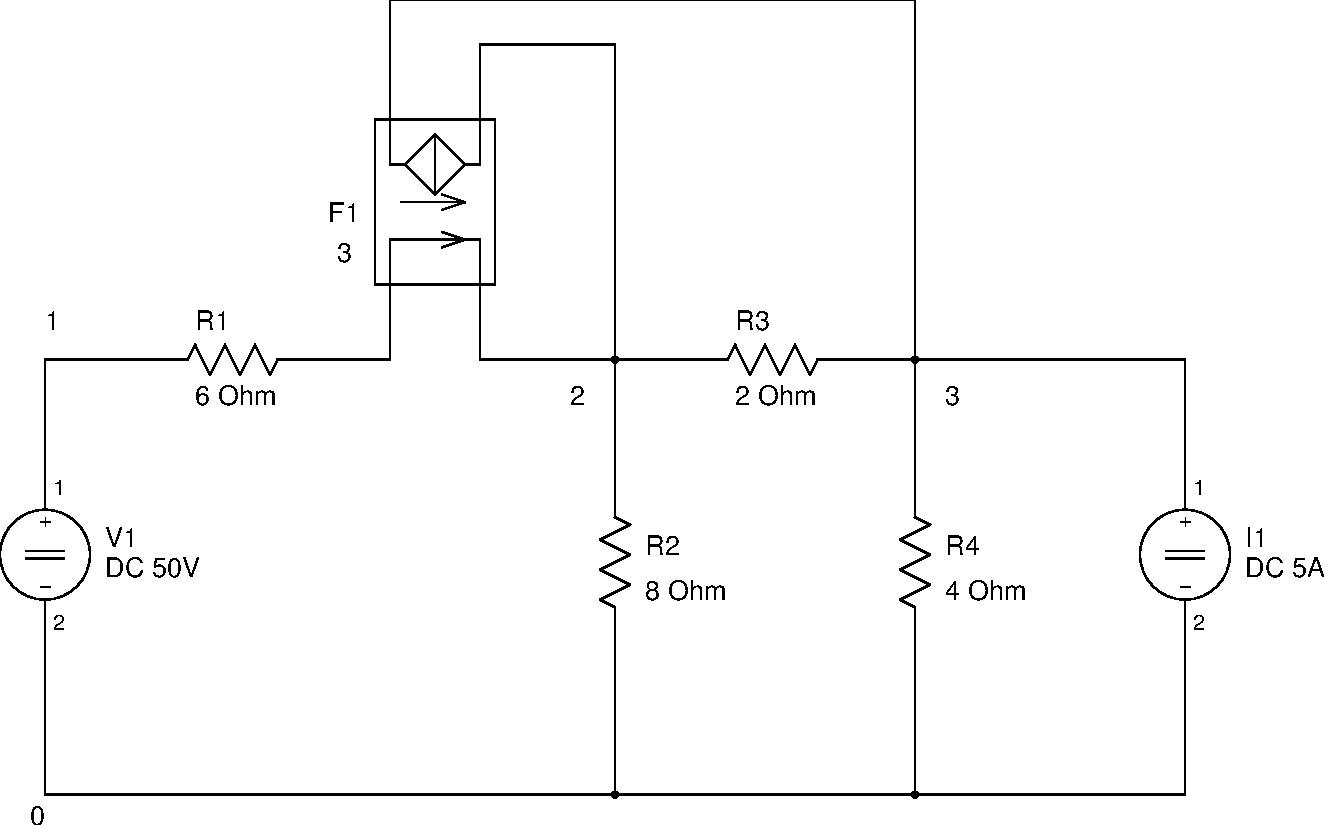
\includegraphics[scale=0.5]{spice/circuit}
\caption{Circuit definition.
Nodes denoted by numbers with 0 as common.
F1 is a current dependent current source, I1 is a current source, and V1 is a voltage source.}
\label{fig:circuit}
\end{figure}

\begin{figure}[!hbtp]
\verbatiminput{spice/circuit.cir}
\caption{SPICE definition of circuit in Figure \ref{fig:circuit}.}
\end{figure}

The simulation can be run using Ngspice with the command:
\begin{verbatim}
  ngspice -b your_file.cir
\end{verbatim}
with \verb+your_file.cir+ replaced by the name of your file
containing the SPICE definition.
To save the output to a file a redirect can be used as
in:
\begin{verbatim}
  ngspice -b your_file.cir > your_file.out
\end{verbatim}
If Orcad is being used the same can be accomplished through
its GUI interface.

\clearpage
% }}}

% {{{ Results
\section{Results}

The output of the simulation is shown in Figure \ref{fig:out}.
Most of the output is extra information about how long the process took
to run and other things that are of no concern in this lab.
The important values are the voltages (\verb+v(1)+, \verb+v(2)+, and \verb+v(3)+).

\begin{figure}[!hbtp]
\verbatiminput{spice/circuit.out}
\caption{Output from SPICE simulation.}
\label{fig:out}
\end{figure}

\clearpage

% }}}

% {{{ Correlation with theory
\section{Correlation with theory}

To correlate the simulation with theory the manual calculations are
performed here and then they are analyzed at the end of this section.

First the node voltage equations
\footnote{For a description of the Node Voltage Method see \cite[Pg. 97]{nilsson2008electric}} are created.
\begin{align}
\frac{v_1 - v_2}{6} &= i_1 \\
v_1 &= 50 \\
\frac{v_1 - v_2}{6} + \frac{-v_2}{8} + \frac{v_3 - v_2}{2} + 3 \cdot i_1 &= 0 \\
\frac{v_2 - v_3}{2} + \frac{-v_3}{4} + 5 - 3 \cdot i_1 &= 0
\end{align}

Simplifying and substituting results in the following set of three equations
with three unknown variables.
\begin{align}
	\frac{1}{2} v_3 - \frac{19}{24} v_2 + 3 i_1 &= -\frac{50}{6} \\
	-\frac{3}{4} v_3 + \frac{1}{2} v_2 - 3 i_1 &= -5 \\
	0 v_3 - \frac{1}{6} v_2 - i_1 &= -\frac{50}{6}
\end{align}

Solving this set of equations results in the following solutions.
\begin{align}
	v_2 &= 32 \quad \mbox{[volts]} \label{eq:v2} \\
	v_3 &= 16 \quad \mbox{[volts]} \label{eq:v3} \\
	i_1 &= 3 \quad \mbox{[amps]}
\end{align}

From the theoretical calculations $v_2 = 32$ volts (Equation \ref{eq:v2})
and $v_3 = 16$ volts (Equation \ref{eq:v3}).
From the SPICE simulation (Figure \ref{fig:out}) $v_2 = 32.0$ volts and
$v_3 = 16.0$ volts.
These values are identical indicating that the theory corresponds
exactly with the simulation.

%\clearpage
% }}}

% {{{ Conclusion
\section{Conclusion}

This experiment was a complete success in performing a detailed
circuit analysis of a circuit with a dependent source by using
both SPICE and manual calculations.
The calculations matched the theoretical values exactly
with no measurable amount of error.

% }}}

% {{{ References
\clearpage

\pagebreak
\renewcommand*{\refname}{\vspace{-8mm}}
\section{References}
\bibliographystyle{ieeetr}
\bibliography{../references}
% }}}

\end{document}

% vim:foldmethod=marker

